\documentclass[10pt, conference]{IEEEtran}
\usepackage{subimages}
\setfigdir{figs}
\usepackage[cmex10]{amsmath}
\interdisplaylinepenalty=2500

\usepackage{amsthm}
\newtheorem{definition}{Definition}

\usepackage{hyperref}

% correct bad hyphenation here
\hyphenation{op-tical net-works semi-conduc-tor}

\usepackage{todonotes}
\usepackage{amssymb}
\usepackage{listings}
\usepackage{balance}

\begin{document}
%
% paper title
% can use linebreaks \\ within to get better formatting as desired
\title{Real Time Eye Gaze Tracking Using Microsoft Kinect}

%------------------------------------------------------------------------- 
% change the % on next lines to produce the final camera-ready version 
\newif\iffinal
\finalfalse
% \finaltrue
\newcommand{\jemsid}{99999}
%------------------------------------------------------------------------- 

% author names and affiliations
% use a multiple column layout for up to two different
% affiliations

\iffinal
  \author{%
    \IEEEauthorblockN{Raul Benites Paradeda}
    \IEEEauthorblockA{%
      INESC-ID \& Instituto Superior T\'{e}cnico\\
      University of Lisbon\\
      Lisbon, Portugal\\
      Email: \href{mailto:raul.paradeda@tecnico.ulisboa.pt}{raul.paradeda@tecnico.ulisboa.pt}}
  \and
    \IEEEauthorblockN{Jones Granatyr, Jean Paul Barddal}
    \IEEEauthorblockA{%
      Graduate Program in Informatics (PPGIa)\\
      Pontif\'{i}cia Universidade Cat\'{o}lica do Paran\'{a} (PUCPR)\\
      Curitiba, Brazil\\
      Email:  \href{mailto:jones.granatyr@pucpr.edu.br}{jones.granatyr@pucpr.edu.br}, \href{mailto:jean.barddal@ppgia.pucpr.br}{jean.barddal@ppgia.pucpr.br}}
   \and
    \IEEEauthorblockN{Alberto Signoretti}
    \IEEEauthorblockA{%
      Graduate Program in Computer Science \\
      State Universtity of Rio Grande do Norte (UERN)\\
      Natal, Brazil\\
      Email:  \href{mailto:albertosignoretti@uern.br}{albertosignoretti@uern.br}}
  }
\else
  \author{Sibgrapi paper ID: \jemsid \\ }
\fi

%------------------------------------------------------------------------- 
% Special Sibgrapi teaser
\teaser{%
  \oneimage{From the left, in the first image it is possible note the lines generated by the gaze estimation, the next figure shows the pre-defined that has an individual timer measuring the time that user gazed to each on, in the third image it is possible see the area of interest created by our method, the next image shows the rectangle created around the eye, and in the last image it is possible observe the result obtained by our method using the clustering algorithm.}{.95}{pic1.png}
}
%------------------------------------------------------------------------- 

% make the title area
\maketitle



\begin{abstract}
	This work presents a technique used to identify in real time, the focus region of the user's gaze through of a Kinect device, and how long the user’s focus is maintained over a specific region of the environment. The technique is divided in two stages. In the first one, the capture of the gaze is performed in two parts, the first one uses predefined regions, and the second is based on regions created using as criteria the user focus of the length of time on each part of the scenario. The second stage performs an algorithm of classification to identify the iris position. As a result, the technique showed that is possible identify and measure how long time the user is gazing to a region and if it is predefined or not. Besides, the log of data related the user's eye were correctly captured and K-means algorithm was performed with success, with real possibilities of allow the correct identification of the iris position.
\end{abstract}

\begin{IEEEkeywords}
	Gaze tracking; Area of interest; Iris tracking.
\end{IEEEkeywords}


\IEEEpeerreviewmaketitle

\section{Introduction}
\todo[inline]{Jean diz: A introducao esta boa. Tem alguns detalhes que vou verificar quando acabar as outras secoes}
	Since the beginning of mankind, vision has became one of the most important senses to stay alive in a harsh environment. 
	In that time, vision was of the utmost importance to survive, create tools, hunt, and adapt to different environments. 
	According to \cite{1} capabilities such as sight became crucial advantage to raise the probabilities of survival in the first ages.
	The sight is so important that, even the eyes have communicative value well before the development of spoken language \cite{2}.
	This assertion is so true that, after the language system has been mastered and made commonplace, eyes are still useful in communication. 
	Eyes send obvious signals with specific messages, such as eye-rolling or subtle winks; or they can be more subtle, such as controlling eye contact to show or withhold intimacy \cite{3}.

	Nowadays, eyes are not only used to create tools or hunt, but mainly as a communication tool in social interaction \cite{4}.
	During communication, one generally does not rely on voice alone, but also on other non-verbal cues, such as body movement, hand movement and gazing, among others.
	Gaze cues are claimed to be used from early life and continue to be given and followed throughout adulthood \cite{4}.
	People have a tendency to orient and follow gaze cues of others and this can be done with relative ease.
	This effect occurs in many situations, ranging from simple aids, as achieve some object, until the attempt to read another player in a poker game, for instance.

	The influence of the gaze that a person has over another is so important that several studies about this subject can be found in academia.
	For example, how gaze cues result in gaze or action following by the observer? 
	The work of \cite{5} describes four studies in which the authors investigated the infant's ability to connect gaze and emotional expression to intentional action.
	In short, this work argues that gazing is a crucial way in which infants recognize the intentional behaviors of other people. 
	The authors obtained this result by repeating an experiment with 8-month, 12-month and 14-month-old children. 
	The experiment was to make that an adult gaze before grasp one of two objects, thereby giving cues. 
	Then, as result they found that at the end of the first year of life, humans better predict the other's actions with the presence of gaze or emotional expression.
    
	Another work is the one by \cite{6}, where authors argued that social conflict is a form of relating and that gaze clues are critical to understanding the underlying cognitive processes in this phenomenon. 
	They showed that by creating an experimental setting that reduces real life to a mixed-motive game, and analyzed the gaze patterns from 22 10- to 12-year-old children in specific game moments that could have been conducted to conflict.
	Authors concluded that children gazes show that they are being more competitive or cooperative at different stages of the game.
	Children avoid confrontation by averting face-directed gazes when asking for larger profits, while gaze longer to attempt to persuade others.

	The present work is a proposition of a tool to automate the evaluation performed during the experiment described in \cite{6}.
	The conclusion of these authors was made manually, i.e. experts watched videos of the children's games play to determine how long each children spent at each gaze to one another.
	To improve this task, we provide a module that is capable of capturing an user's gaze and automatically measures the time of each gaze.
	Using angles provided by Microsoft Kinect and vector formulas, we capture the user's gaze and its duration.
	Additionally, the automated tool also captured and read information about users' eyes region and created a dataset composed of color information and coordinates.
	Afterwards, it will be necessary to apply a clustering algorithm to identify regions and similarities. 

	This paper is organized as follows.
	In Section \ref{sec:relatedWork} we present related works that uses Microsoft Kinect to identify user gaze.
	Later, Section \ref{sec:technologyUsed} describes the two versions of Microsoft Kinect.
	Section \ref{sec:eyeGazeEstimation} describes our proposal for eye gaze identification and length measuring, while Section \ref{sec:dataExtraction} discusses around data extraction.
	Finally, Section \ref{sec:conclusionAndFutureWork} sums up this paper and puts forward future work.

\section{Related Work} \label{sec:relatedWork}

	\todo[inline]{Jean diz: Favor verificar algumas duvidas e se as referencias estao ok}
	In work of \cite{7}, authors proposed a system that adopts a personalized 3D face model along with an eye detection gaze through iris using the first version of Microsoft Kinect. 
	To identify the iris they ran the Starburst algorithm \cite{8} with some modifications. 
	This experiment was performed starting with the calibration phase, where the participants should look to nine predefined points in the screen and several images were taken of the participant face for each point observed. 
	Then, to the phase of gaze estimation, participants were asked to gaze to a predefined point. 
	After one session, each participant was asked to move his/her seat position before starting the next step. 
	They performed this method several times aiming at collecting the data that was used to calibrate the system.
	According to the results, the authors concluded that Microsoft Kinect provides more accurate gaze estimation compared with RGB images and their calibration mode reduced the degree of the error.
	\todo[inline]{better results were achieved with rgb instead of some other color space? is that it?}
    \todo[inline]{Não, os melhores resultados foram obtidos utilizando as imagens originadas do Kinect, em comparação com outras imagens}

	In other work, authors in \cite{8} used a system to calibrate the iris position using the nine points method \cite{9}, which randomizes some points in the screen and asks the user to gaze each point, one by one. 
	\todo[inline]{I could not understand the next sentence}
    \todo[inline]{Os autores dividiram em dois grupos, o local e o global. Local eles se baseiam apenas na posição da iris, enquanto que o local é baseado em relação ao movimento da cabeça.}
	Their tests embedded two scenarios: the first one consisted of separating the gaze motion in local motion, while the second one aimed at separating it in global motion. 
	According to them, the local motion refers to the gaze motion driven by pupil movement and the global motion is related to motion driven by head movement. 
	The authors compared their results with the work of \cite{9} \todo{are these citations correct?} \todo{yes} and they proposed method performs exceptionally well for the reliability and precision in gaze identification.

	In turn, authors in \cite{10} proposed a method to estimate the gaze direction in a 3D space with the first version of Microsoft Kinect. 
	The authors combined depth and visual data to create texture 3D mesh of the scene. 
	Besides, parameters of head-pose were used to stabilize the 3D scene and to generate eye images. 
	As a result, authors could estimate the gaze direction under challenging head poses and low-resolution eye images.

\section{Microsoft Kinect} \label{sec:technologyUsed}
	\todo[inline]{Jean diz: Secao esta ok}
    
	As previously mentioned, the Microsoft Kinect device was used to provide the necessary information for gaze identification.
	This section aims to discuss some important differences between the first and the second version of this device.
	This is particularly important because most of the related works used the first version, and the new resources implemented on the current version can improve the overall performance of the device.

	This device has an infrared projector, cameras and a special microchip to track the movement of objects and people in three dimensions. 
	Furthermore, it has a 3D depth sensor, tilt motor and microphones.
	The second version received some improvements when compared to the first version. 
	For example, the first version of Kinect has a color image resolution of 640 x 480 pixels with a field of view (fov) of 62 x 48.6 degrees, which results in an average of about 10 x 10 pixels per degree. 
	On the other hand, the second version of Kinect presents color image resolution of 1920 x 1080 pixels and a fov of 84.1 x 53.8, resulting in an average of about 22 x 20 pixels per degree. 
	The improvements imply in better image quality, thus, possibly making better detection of data contained in retrieved images.

	Another important difference is in the depth image, where the Kinect v1 has a resolution of 320 x 240 pixels with a fov of 58.5 x 46.6 degrees resulting in an average of about 5 x 5 pixels per degree. 
	Conversely, the Kinect v2 has a depth image resolution of 512 x 424 pixels with a fov of 70.6 x 60 degrees resulting in an average of about 7 x 7 pixels per degree. 

	According to Microsoft specifications for Kinect for Windows, the Kinect v2 face recognition, motion tracking and resolution are much more precise than the Kinect v1. 
    Kinect v2 uses ``time of flight'' technology to determine the features and motion of certain objects. 
	Besides, the v2 can process 2 gigabytes of data per second, the adopted USB 3.0 provides almost ten times faster broadband for the data transfer, 60\% wider field of vision, and it can detect and track 20 joints from 6 people’s bodies including thumbs. 
	Besides, when using Kinect v2 is possible to detect heart rates, facial expressions and weights on limbs, along with much more extremely valuable biometric data, as one can see in Fig. \ref{fig:fig2}.

    \begin{figure}[t]
        \centering
        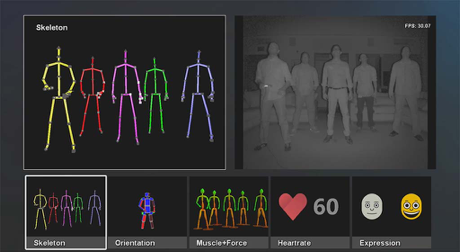
\includegraphics{figures/pic2.png}
        \caption{Kinect v2 detections.}
        \label{fig:fig2}
    \end{figure}

	Given the improvements provided by Microsoft Kinect v2, our experiments were ran on top of it mainly because of higher image quality, reliability and precision regarding face position.
	Another important trait of our project is the integration of Microsoft Kinect with its respective Software Development Kit (SDK) to compute some important values to the developer, as well as the width and height, in pixels, of some object on the screen.
    These values are returned by the methods of \emph{KinectSensor} object, namely \emph{ColorFrameSource} and \emph{DepthFrameSource}.
	Therewith, it is possible to set some regions such as user's head, and retrieve the width, height, and his angle.

	However, for the purpose of this work another class of the SDK Kinect is more important, named \emph{Kinect.Face}. 
	Using this class, it is possible to capture some interesting information, such as: rotation orientation, face engagement, glasses, happy, is left eye closed, is right eye closed, is looking away, has mouth moved, and is mouth open. 
	These values can be seen in Fig. \ref{fig:fig3}, where it is possible to note the information available in the screen provided by the \emph{Kinect.Face} method.

    \begin{figure}[t]
        \centering
        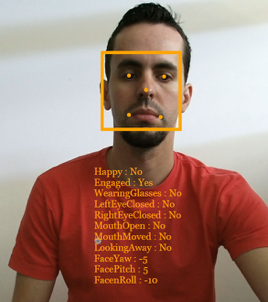
\includegraphics{figures/pic3.png}
        \caption{Information provided by \emph{Kinect.Face} method.}
        \label{fig:fig3}
    \end{figure}

\section{Eye-Gaze Estimation} \label{sec:eyeGazeEstimation}

	The rotation orientation is important to determine the vector and tracing of a gaze line. 
	This orientation is informed by the \emph{Kinect.Face} method and its values represent the axis $X$, $Y$ and $Z$, related to the user face rotation. 
	However, the values returned by the method are in a system number called ``quaternions'', and the values refer to, pitch (rotation about the X-axis), yaw (rotation about the Y-axis) and roll (rotation about the Z-axis) (see Fig. \ref{fig:fig4}). 
	Quaternions are mathematical structures that combine complex numbers and vector concepts \cite{2,11} that can be named as hyper-complex numbers or fourth dimension vectors. 
	The quaternions formula is given by Equation \ref{eq:quaternion}, where $a$, $b$, $c$ and $d$ are real numbers and $i$, $j$ and $k$ are basis elements of $H$.
    
    \begin{equation}
		H = \{a+ bi + cj + dk ~ \vert ~ a, b, c, d \in \mathbb{R} \}
        \label{eq:quaternion}
	\end{equation}

\begin{figure}[t]
	\centering
	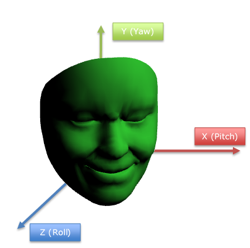
\includegraphics{figures/pic4.png}
    \caption{Quaternions returned by Kinect.Face method and their vertices.}
    \label{fig:fig4}
\end{figure}

	Therefore, the quaternions values are used to calculate the Euler angles. 
	The Euler angles are three angles introduced by Leonhard Euler to describe the orientation of a rigid body, which is a body in which the relative position of all its points is constant \cite{12}. 
	Nevertheless, in this project the Euler angle must be given in degrees.
    This conversion allows the prediction of the target of an user's gaze.
	The conversion code that transform the Euler values to degrees can be seen in the following code snippet, where the $y$, $w$, and $z$ variables represent the angles provided by Kinect sensor and $yawD$, $pitchD$ and $rollD$ are variables that will receive the values representing the degrees after the conversion.
    
\todo[inline]{Acho que isso seria melhor descrito por equacoes.}
\todo[inline]{Concordo}
\begin{lstlisting}
double yawD, pitchD, rollD;
pitchD = Math.Atan2(2*((y*z)+(w*x)),
		 (w*w)-(x*x)-(y*y)+(z*z))
         /Math.PI*180.0;
yawD = Math.Asin(2*((w*y)-(x*z)))
		/Math.PI*180.0;
rollD = Math.Atan2(2*((x*y)+(w*z)),
		(w*w)+(x*x)-(y*y)-(z*z))
        /Math.PI*180.0;
\end{lstlisting}

	After the conversion, it is possible to calculate the heading vector. 
	One of the objective of this work is to trace a line from each point located in user face, such as: one point in each eye, one in the nose and one in each side of the mouth, as shown in Fig. \ref{fig:fig5}. 
	From these points, a line will be generated based on the angle of user head \todo[inline]{frase incompleta?}\todo[inline]{Veja se ficou mais claro}. 
	Therefore, to trace the line for each point in the system screen is necessary two points: begin point and end point, both provided in the pixels format). 
	The begin point is determined by the points in user face and the end point must be calculated from the angle of user head. 
	To calculate the end point a normalization is necessary to inform the orientation of the angles, informed by the \emph{Kinect.Face} method. 
	The normalization was performed given Equations \ref{eq:normalizationX} and \ref{eq:normalizationY}, where $X$ is the pitch and $Y$, both provided by \emph{Kinect.Face}.
    \begin{equation}
    	normX = \frac{X}{\sqrt{X^2 + Y^2}}
		\label{eq:normalizationX}
	\end{equation}
    \begin{equation}
    	normY = \frac{Y}{\sqrt{X^2 + Y^2}}    
		\label{eq:normalizationY}
	\end{equation}

    \begin{figure}[t]
        \centering
        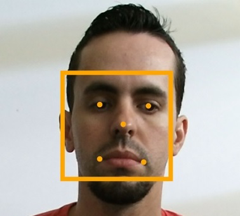
\includegraphics{figures/pic5.png}
        \caption{Predefined face points.}
        \label{fig:fig5}
    \end{figure}

	After the normalization, the angle was converted into a vector by applying the arc cosine formula and converting the angle from degress to radians.
	Equation \ref{eq:pitchTransformation} depicts the transformation to the pitch value, where $\arccos$ is the inverse cosine function and $normX$ is the normalized pitch angle.
    \todo[inline]{nao eh necessario realizar essa conversao para as outras componentes, i.e. yaw e roll?}
    \todo[inline]{não, pois para o objetivo do projeto aqueles angulos não interessa a conversão.}
	\begin{equation}
    	P = \arccos{(normX)} \times \frac{180}{\pi}
		\label{eq:pitchTransformation}
	\end{equation}
	
    \todo[inline]{a definicao do end point nao esta nem um pouco clara}
    \todo[inline]{para gerar uma linha é necessário dois pontos, um de inicio e um de fim. O de inicio é informado pelo kinect, e o ponto final é o valor de P (se eu não me engano) hehe}
	Finally, after this process these values were used to mark the end point of the line. 
	In short, the begin point is provided by SDK Kinect through the method \emph{Kinect.Face} and the end point was calculated after a series of formulas and conversions starting from the quaternions. 
	In Fig. \ref{fig:fig6} it is possible to visualize the line generated by the angle of user head at each head move. 
	In the first image, it is possible note that the user tilted the head to the left and were created lines predicting where the user gaze is. 
	This effect happens in the other images, where lines predicting the user gaze were created according to the tilt of user head.

  \begin{figure}[t]
      \centering
      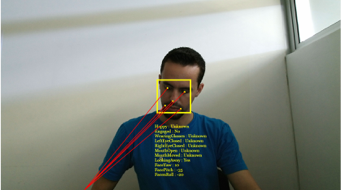
\includegraphics{figures/pic6a.png}\\
      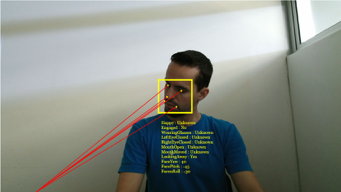
\includegraphics{figures/pic6b.png}\\
      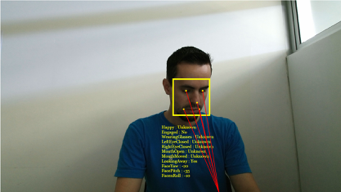
\includegraphics{figures/pic6c.png}\\
      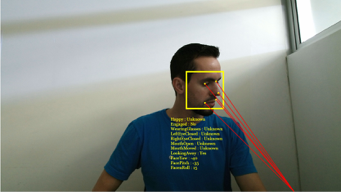
\includegraphics{figures/pic6d.png}
      \caption{Line determined by the head angle and simulating the user gaze.}
      \label{fig:fig6}
  \end{figure}

\subsection{Predefined Areas}

	As mentioned earlier on this paper, this work is an extension of \cite{6}, so it is necessary to define the regions where will be measure the time of the user gaze in each of these regions. 
	The experiment accomplished in Campos was a game with cards. 
	Because of that, the region where the players will gaze is under his head (on the table) and to the other player, located in front of him. 
	Thus, we defined in this project four regions on the bottom of the screen (simulating the cards positions) and one on middle of the screen (simulating the other player), as we can see in Fig. \ref{fig:fig7}.

  \begin{figure}[t]
      \centering
      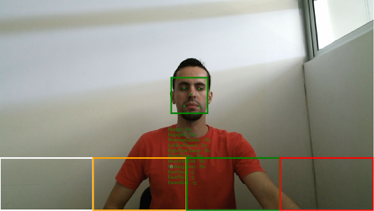
\includegraphics{figures/pic7.png}
      \caption{Regions predefined simulating the cards and other player.}
      \label{fig:fig7}
  \end{figure}

	After determining the important areas for this purpose, it is necessary to calculate the time where the gaze of user is on each one of these areas. 
	Thus, we created a method that starts a timer for each region when the end point of the gaze line reaches some region. 
	The time for each region is stored in an array, in which each position represents an observed area. 
	The time that the user gaze in each region is represented as a text on the left corner inside of each region, as we can see in Fig. \ref{fig:fig8}. 
	When the experiment is over, the time for each region is outputted to text files for future studies.

    \begin{figure}[t]
        \centering
        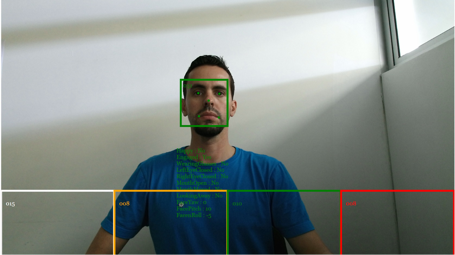
\includegraphics{figures/pic8.png}
        \caption{Seconds observed in each region represented on the left corner of each region.}
        \label{fig:fig8}
    \end{figure}
	\todo[inline]{Jean diz: li ate aqui}
\subsection{Non-predefined Areas}

The first step of this work showed that it is possible to capture the time and the region where the user is gazing. 
However, in some cases the experience do not have a pre-defined area and the system must be able to recognize any special area that has the user attention. 
Because of that, a second prototype was made, where the system recognize an area that was gazing by the user. 
Afterwards, we built a rectangle and counted the seconds that the user is gazing for this area (Fig. \ref{fig:fig9}). 
This area is considered important when the user gaze at least for 2 seconds. 
When there is a change of gaze to another point of interest and at least for 2 seconds, another region is built. 
As can be noted in Fig. \ref{fig:fig9}, in the first image the user gazed to a non-specific position at least by 2 seconds, and the system identified that can be an area of interest and created a square. 
Then, in the other image, the user gazed to another position at least by 2 seconds, and the system created another area of interest. 
Whether the gaze is in a region, which was previously defined, the timer continues where it left off.

\begin{figure}[t]
	\centering
	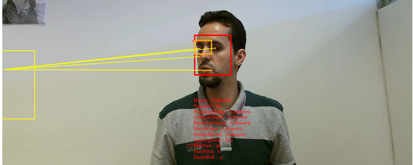
\includegraphics{figures/pic9a.png}\\
    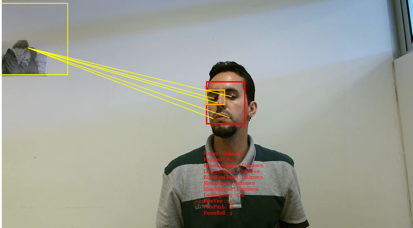
\includegraphics{figures/pic9b.png}\\    
    \caption{Area of interest defined by the system.}
    \label{fig:fig9}
\end{figure}

	However, this method uses the head position and it can be a problem. 
	For example, the user can turn the head to the left but your gaze is on the center. 
	It can happen because of the iris position, and for this reason it is necessary a future study about how to capture the iris position. 
	On the next section we explain the performed tests to reach this goal.

\section{Data Extraction} \label{sec:dataExtraction}

	After the identification of the region where the user could be gazing, it was necessary to develop a more accurate system. 
	This system aims to identify user’s iris and predict with more precision the region where is the gaze. 
	To reach this goal, firstly it was necessary to define the user eye region to collect the data provided by the Kinect device.
	In our prototype, were captured the data of one eye. 
	It was done because the capturing process related to all data provided by Microsoft Kinect is impractical. 
	It happens because there are a great amount of unnecessary information to the project, then, from the point created by Kinect above the user eye, it was created a rectangle (Fig. \ref{fig:fig10}) to visualize what is the region being captured. 
	In this sense, the unnecessary information was reduced, i.e., only information regarding the eyes were captured.

  \begin{figure}[t]
      \centering
      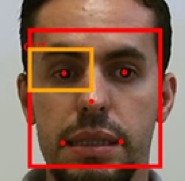
\includegraphics{figures/pic10.png}
      \caption{Eye region identified by the yellow rectangle.}
      \label{fig:fig10}
  \end{figure}

	Using the rectangle coordinates around the eye, it is possible to read a lot of information, as, the position of each pixel in the screen, the color of each pixel, depth of each pixel, values of luminosity, values of infrared, etc. 
	However, only values that allow the system to make possible to identify the iris of the user inside of this region, were read in our experiments: R (red), G (green), B (blue), A (alpha control color opacity), Hex (hexadecimal value color), POS (pixel position inside of pixel array available by Kinect), X and Y (coordinate X and Y of pixel).
	These data were obtained from an array that is available by the Kinect device. This array has 8294400 positions, independently of the resolution of the display. 
	It is defined by the multiplication of the Kinect camera resolution (1920 * 1080) and this result is multiplied by four (representing R, G, B and A values). 
	Thereby, each position represent a color or opacity value. Each screen line is represented by 7680 array positions, also not mattering the screen resolution. In other words, the first 7680 array positions represent colors and opacity of the first line of pixels of the screen (Fig. \ref{fig:fig11}). 
	This value is obtained by dividing the total of the array positions for the resolution of Kinect camera, which is 1080p. 
	As mentioned before, each pixel of the screen is represented by four positions of the array, exemplifying, the 0, 1, 2 and 3 position of the array represent the pixel located in position 0x0 (X and Y) in screen coordinates, and the positions 4, 5, 6 and 7 of the array represent the pixel in position 0x1 (X and Y) in screen coordinates, and so forth.
	This approach to color representation used in Kinect presents some difficulties, such as the size of the array is constant independently of the screen resolution. 
	The problem happens because of the position of determined pixels in a 1920 x 1080 screen resolution, so the set of four indices in array (that represent these pixels), will be different in other resolution. 
	For example, if we have the following positions: X = 10 and Y = 0 (first row tenth pixel) at a 1920 x 1080 resolution, it will read the values 40, 41, 42 and 43 of index position of array. On the other hand, in a 800 x 600 resolution the values in array that will be read are: 96, 97, 98 and 99 index position of array. 
	Due to this fact, it was necessary to create a heuristic that allows the reading of the correct positions of the array, regardless of display resolution.

  \begin{figure}[t]
      \centering
      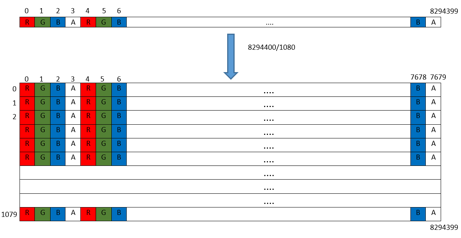
\includegraphics{figures/pic11.png}
      \caption{Representation of color array available by Kinect device.}
      \label{fig:fig11}
  \end{figure}

	Thereby, to capture the information inside the rectangle created around the user eye (Fig. \ref{fig:fig10}), it was necessary to identify which array index each border was being represented inside of array that represent the screen (Fig. \ref{fig:fig12}), regardless of display resolution. 
	This it is necessary because the array available by Kinect, as mentioned, has 8294400 positions, representing the color of each pixel in the screen, but we just need the positions that represent the user eye. 
	As can be seen in Fig. \ref{fig:fig12}, it is necessary search in the array the index that represent each border of the screen. 
	At a first moment, it was necessary to determine an adjustment variable named sigma, which is calculated as follows:
double sigma=(double)1080-actualHeight) / actualHeight;

where:
	sigma: adjustment variable;
	actualHeight: height in pixels of the display resolution.

After the sigma is calculated, it is necessary identify in which axis (X or Y) each rectangle line is positioned, as follows:
int correctFCPTop=(int)faceBoxPosition.Top*actualHeight/1080;
int correctFCPRight=(int)faceBoxPosition.Right*actualWidth/1920;
int correctFCPBot=(int)faceBoxPosition.Bottom*actualHeight/1080;
int correctFCPLeft=(int)faceBoxPosition.Left*actualWidth/1920;

where:
	actualHeight: height in pixels of the display resolution;
	actualWidth: width in pixels of the display resolution;
	faceBoxPosition.Top: most on the top position on axis Y;
	faceBoxPosition.Right: most on the right position on axis X
	faceBoxPosition.Bottom: most on the bottom position on axis Y.
	faceBoxPosition.Left: most on the left position on axis X;

  \begin{figure}[t]
      \centering
      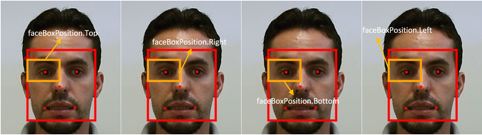
\includegraphics{figures/pic12.png}
      \caption{Indicating the face box position.}
      \label{fig:fig12}
  \end{figure}

	After the retrieval of the coordinates, it is identified which index of array colors that each rectangle corner represents.
	To reach this goal it was necessary to execute the Code 2. 
	In this code, to find determined point, for example, the point that represent on the left on the top of the rectangle, was necessary multiple the value that define the border on the left (correctFCPLeft) by the resolution of the screen (1920). 
	With this result, divide by the width screen. Then, multiply by 4, because is four fields (values of R, G, B and A). 
	Finally for this point, it is necessary sum this result with the result of the next operation, that is, multiply the 7680 value (that is the number of index in one row of the array) by the sum of the number that represent the top position (correctFCPTop) with this same value, but truncated, multiplied with the sigma value.

\todo[inline]{Equations}
Code 2: Calculate the array index that represent each corner of the rectangle.
\begin{lstlisting}
initialPointTop = Convert.ToInt64(Math.Truncate(((((int)correctFCPLeft * 1920) / actualWidth) * 4) + (7680 * ((int)correctFCPTop + Math.Truncate((int)correctFCPTop * sigma)))));
finalPointTop = Convert.ToInt64(Math.Truncate(((((int)correctFCPRight * 1920) / actualWidth) * 4) + (7680 * ((int)correctFCPTop + Math.Truncate((int)correctFCPTop * sigma)))));
initialPointBot = Convert.ToInt64(Math.Truncate(((((int)correctFCPLeft * 1920) / actualWidth) * 4) + (7680 * ((int)correctFCPBot + Math.Truncate((int)correctFCPBot * sigma)))));
finalPointBot = Convert.ToInt64(Math.Truncate(((((int)correctFCPRight * 1920) / actualWidth) * 4) + (7680 * ((int)correctFCPBot + Math.Truncate((int)correctFCPBot * sigma)))));
\end{lstlisting}


	Finally, after found the index in the array that represent the border of the rectangle around the user eye, all values inside of this rectangle were read and written in a text file. 

	To validate if the capture of the values were in a correct way, it was generated an image from the data of this text file. 
	In this way, once can be see that the capture was done in a way that is possible identify the user eye, as can be seen in Fig \ref{fig:fig13}.

    \begin{figure}[t]
      \centering
      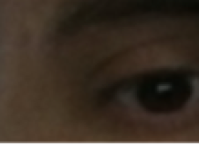
\includegraphics{figures/pic13.png}
      \caption{Image created based on the data in the text file.}
      \label{fig:fig13}
    \end{figure}

\subsection{Clustering}

	With the text file created in the extraction data step, it was used a clustering algorithm called K-Means \cite{13}. 
	This algorithm use a simple and easy way to group a given data set through a certain number of clusters (assume k clusters) fixed a priori. 
	The main idea is to define k centroids, one for each cluster. 
	These centroids can be placed using some methodologies because of its location, depending upon the results may be different. 
	In this way, one choice is to place them as much as possible far away from each other. 
	The next step is to take each point belonging to a given dataset and associate it to the nearest centroid. 
    When no point is pending, the first step is completed and an early groupage is done. 
	At this point, we need to re-calculate the k new centroids as barycenter’s of the clusters resulting from the previous step. 
	After we have these k new centroids, a new binding has to be done between the same data set points and the nearest new centroid. 
	A loop is generated and as a result, we may notice that the k centroids change their location step by step until no more changes are done. 
	In other words, centroids do not move any more.
	Although it can be proved that the procedure will always terminate, the k-means algorithm does not necessarily find the most optimal configuration. 
	The algorithm is also significantly sensitive to the initial randomly selected cluster centers. 
	The k-means algorithm can be run multiple times to reduce this effect.
	In short, this algorithm has a characteristic to try to find similarities between examples and then put a classification in these (cluster number). 
	The main idea is attempt to find the user iris based on the classification made by this clustering algorithm. 
	Therefore, we have made tests using the k value equal 2, 3, 4, 5, 10 and 15, and its results can be seen in Fig \ref{fig:fig14}.
	As can be seen in Fig \ref{fig:fig14}, in all tests there are possibilities to identify the iris position for the reason that the examples that identify the iris are in at least one cluster. 
\todo[inline]{Está faltando as outras imagens que fazem parte dessa figura.}
\begin{figure}[t]
	\centering
	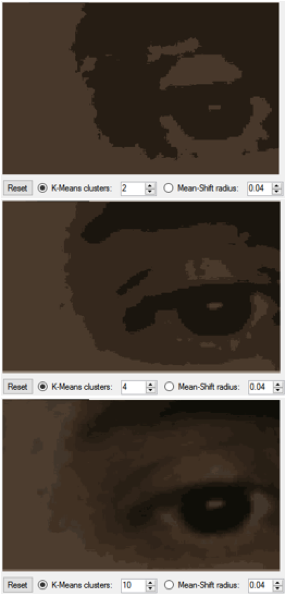
\includegraphics{figures/pic14.png}
    \caption{K-Means test results, at top left was used K = 2, on right K = 3, next, K = 4, K = 5, K = 10 and finally K = 15.}
    \label{fig:fig14}
\end{figure}

\section{Conclusion and Future Work} \label{sec:conclusionAndFutureWork}
\todo[inline]{Jean diz: conclusao esta quase ok tb}
	Some clues (such as pointing, gaze and language) are important to make the observer do what is desired. 
	In some scenarios, some clues are more important than others, e.g. autism.
	Children with autism are known to have difficulties in sharing attention with others, while some researches \cite{14} show that a reasonable proportion of autistic children do not show difficulties in following another's head turn.
	Gaze is important to identify what one desires, mainly in cases where one is unable to talk or indicate, e.g. cases of infants and people with disabilities.
	Still, in cases such as in Campus work where the gaze was used in a game context and identified that the children tend to avoid confrontation by averting face-directed gazes when they are asking for something, and they gaze longer to attempt to persuade one another.

	Our proposal is relevant to aid experiments where there is the need to identify the user gaze in real time and its duration at each region, all given by its head angle.
	Moreover, it was possible to create regions of interests according to the length of gazes towards some region, regardless these were predefined or not.
	Nevertheless, we identified some problems with the use of this technique solely using head positions. 
	One of them is if the head position is slightly tilted to a side, the user could be gazing to the contrary side or the center. 
	This can happen because of his iris position. 
	Because of that, in this first prototype an image was created from the data of each pixel of the eye region that was informed by the Microsoft Kinect device, showing that the data collected were correct. 

	Next, to improve the used technique, k-means clustering was performed to predict the user iris position. 
	This algorithm received as input the data which represent the user eye, and then the clusters were created according with similarity of each pixel. 
	Based on that, it was possible to perceive that the user iris, depending of the number of clusters, can be easily identified.
	As future work, we intend to make the identification of the data that represent the user iris, in an automatic and real time way. 
	This would allow a more accurate prediction of user gaze independently of head angle.
	\todo[inline]{Again, this is not clear if you used or not the iris positioning}
    \todo[inline]{O uso da posição da Iris para determinar para onde o usuário está olhando é para os trabalhos futuros.}


\bibliographystyle{IEEEtran}
\balance
\bibliography{example}
\balance

\end{document}
